\documentclass[letterpaper]{article} % DO NOT CHANGE THIS
\usepackage[submission]{aaai2027} % DO NOT CHANGE THIS
\usepackage[hyphens]{url} % DO NOT CHANGE THIS
\usepackage{graphicx} % DO NOT CHANGE THIS
\urlstyle{rm} % DO NOT CHANGE THIS
\def\UrlFont{\rm} % DO NOT CHANGE THIS
\usepackage{natbib} % DO NOT CHANGE THIS AND DO NOT ADD OPTIONS
\usepackage{caption} % DO NOT CHANGE THIS AND DO NOT ADD OPTIONS
\frenchspacing % DO NOT CHANGE THIS

\usepackage{booktabs}
\usepackage{amsmath}
\usepackage{amssymb}

\pdfinfo{
/TemplateVersion (2027.1)
}

\setcounter{secnumdepth}{2}

\title{Beyond Weight Geometry: Tracking On-Policy Distillation with Domain-Conditioned Functional Spectra\\Supplementary Material}
\author{Anonymous Submission}
\affiliations{}

\begin{document}
\maketitle
\appendix

\section{Mathematical Foundations}

\subsection{Whitened Coordinates Represent the Same Weight Map}

Fix a checkpoint, domain, and linear module. Write
\begin{equation}
\Sigma=\mathbb E[hh^\top],\qquad S=\Sigma^{1/2},\qquad A=WS,
\end{equation}
where $h\in L^2(\Omega;\mathbb R^d)$, $W\in\mathbb R^{m\times d}$, $S$ is the
symmetric positive-semidefinite square root, and $S^\dagger$ is its
Moore--Penrose pseudoinverse. Let $z=S^\dagger h$ and
$P=S^\dagger S$, the orthogonal projector onto $\operatorname{range}(\Sigma)$.
For every member $v_j$ of a finite orthonormal basis of $\ker(\Sigma)$,
$\mathbb E[(v_j^\top h)^2]=v_j^\top\Sigma v_j=0$, so $v_j^\top h=0$ almost
surely. Intersecting these finitely many probability-one events shows that $h$
lies in $\ker(\Sigma)^\perp=\operatorname{range}(S)$ almost surely. It follows that
\begin{equation}
h=Sz,\qquad \mathbb E[zz^\top]=P,\qquad Wh=WSz.
\label{eq:supp-whiten}
\end{equation}
Within the support of $\Sigma$, $P$ is the identity. Thus $WS$ is not a separate
activation model: it is the original weight map written in domain-conditioned whitened
input coordinates.

\subsection{Output Second Moment and Optimal Approximation}

For the module output $y=Wh$,
\begin{equation}
AA^\top=W\Sigma W^\top=\mathbb E[yy^\top].
\label{eq:supp-output}
\end{equation}
Therefore $\sigma_i^2(A)$ is the $i$th eigenvalue of the module-output second moment and
$\|A\|_F^2=\mathbb E\|y\|_2^2$. For any candidate weight $\widetilde W$,
\begin{equation}
\mathbb E\|(W-\widetilde W)h\|_2^2
=\|(W-\widetilde W)S\|_F^2.
\label{eq:supp-error}
\end{equation}
Let $A_r$ be the rank-$r$ truncated SVD of $A$. Since the nonzero right singular
directions of $A=WS$ lie in $\operatorname{range}(S)$, choosing
$\widetilde W_r=A_rS^\dagger$ gives
$\operatorname{rank}(\widetilde W_r)\leq\operatorname{rank}(A_r)\leq r$ and
$\widetilde W_rS=A_r$. Conversely, every
$\operatorname{rank}(\widetilde W)\leq r$ produces
$\operatorname{rank}(\widetilde WS)\leq r$. The Eckart--Young--Mirsky lower
bound applies to this latter matrix, while $\widetilde W_r$ attains it. Hence
\begin{equation}
\min_{\operatorname{rank}(\widetilde W)\le r}
\mathbb E\|(W-\widetilde W)h\|_2^2
=\sum_{i>r}\sigma_i^2(A).
\label{eq:supp-optimal}
\end{equation}
Consequently, $r_\varepsilon(WS)$ is the minimum rank whose optimal approximation loses
at most an $\varepsilon$ fraction of expected module-output energy. We define
$r_\varepsilon(0)=0$.

\subsection{Coordinate Invariance}

For an invertible input reparameterization $h'=Th$, define
$W'=WT^{-1}$ and $\Sigma'=T\Sigma T^\top$. For any factor $S'$ satisfying
$S'(S')^\top=\Sigma'$,
\begin{equation}
(W'S')(W'S')^\top
=W'\Sigma'(W')^\top
=W\Sigma W^\top.
\end{equation}
Thus $W'S'$ and $WS$ have the same nonzero singular values. An invertible rescaling can
change the bare-weight spectrum while leaving the functional spectrum unchanged. This is
the formal scale correction used in the paper.

\subsection{Current, Fixed, and Centered Input Metrics}

The main construct uses the current moment, $W_tS_{D,t}$. Fixed whitening,
$W_tS_{D,0}$, places every checkpoint on the base input metric. The exact identity
\begin{equation}
W_tS_t-W_0S_0
=(W_t-W_0)S_0+W_t(S_t-S_0)
\label{eq:supp-fixed}
\end{equation}
does not create a causal decomposition: $S_t$ is an endogenous result of the current
model, and $r_\varepsilon$ is nonlinear. Fixed whitening is therefore a sensitivity
audit, not an estimate of ``the fraction caused by activations.''

The centered audit replaces $\Sigma$ by
\begin{equation}
\Sigma^{\mathrm c}
=\mathbb E[(h-\mathbb E h)(h-\mathbb E h)^\top].
\end{equation}
It removes the activation-mean direction and changes the estimand from output second
moment to output covariance. It is reported as a boundary check rather than as the
primary definition.

\subsection{Discrete and Continuous Spectral Stability}

If $\widetilde A=A+E$, Weyl's inequality gives
$|\sigma_i(\widetilde A)-\sigma_i(A)|\le\|E\|_2$. A direct sufficient
condition for stability follows from the best rank-$j$ residual
\begin{equation}
T_j(A)=\min_{\operatorname{rank}(X)\leq j}\|A-X\|_F^2
=\sum_{i>j}\sigma_i^2(A).
\end{equation}
Let $F=\|A\|_F$, $e=\|E\|_F$, and $b=2Fe+e^2$. The distance to the
rank-$j$ set is 1-Lipschitz in Frobenius norm, which gives
$|T_j(\widetilde A)-T_j(A)|\leq b$; likewise
$|\|\widetilde A\|_F^2-F^2|\leq b$. For $r\geq1$ and $b<F^2$, the two
inequalities
\begin{equation}
\frac{T_r(A)+b}{F^2-b}\leq\varepsilon,\qquad
\frac{T_{r-1}(A)-b}{F^2+b}>\varepsilon
\label{eq:supp-rank-stability}
\end{equation}
therefore imply $r_\varepsilon(\widetilde A)=r_\varepsilon(A)=r$.
The condition is sufficient rather than necessary, but makes explicit why a discrete
rank may move by a few directions when an adjacent tail ratio is close to
$\varepsilon$. We consequently repeat the analysis with
$\varepsilon\in\{.01,.025,.05,.10\}$ and with
\begin{align}
r_{\mathrm{stable}}(A)&=\frac{\|A\|_F^2}{\|A\|_2^2},\\
r_{\mathrm{ent}}(A)&=\exp\left(-\sum_i p_i\log p_i\right),
\quad p_i=\frac{\sigma_i^2}{\sum_j\sigma_j^2}.
\end{align}
For the zero matrix, we set
$r_{\mathrm{stable}}(0)=r_{\mathrm{ent}}(0)=0$ and use the convention
$0\log 0=0$.
These continuous summaries test whether an ordering is an artifact of one threshold.

\section{Experimental and Estimation Protocols}

\subsection{Training Settings and Checkpoint Intersections}

The two students are Qwen3-4B-Base and Llama-3.2-3B. All settings use rank-32 LoRA.
OPD uses current-student rollouts with teacher forward KL; off-KD uses frozen teacher
sequences with the same soft objective; seqKD uses the exact off-KD sequence stream and
order with hard next-token targets; SFT uses external reference chains of thought.
Qwen additionally includes $\alpha=.5$ current-self exposure, and Llama includes
frozenSelf0-KD, which permanently reuses rollouts generated by the step-0 student.

\begin{table}[t]
\centering
\small
\setlength{\tabcolsep}{3.5pt}
\begin{tabular}{lccc}
\toprule
Setting & Sequence producer & Refreshed & Target \\
\midrule
OPD & current student & yes & teacher KL \\
$\alpha=.5$ & mixed support & yes & teacher KL \\
frozenSelf0 & step-0 student & no & teacher KL \\
off-KD & teacher & no & teacher KL \\
seqKD & teacher & no & hard CE \\
SFT & external reference & no & hard CE \\
\bottomrule
\end{tabular}
\caption{Control variables represented by the training settings. Not every auxiliary setting is
available for both models. Main comparisons use strict checkpoint intersections and never
interpolate missing checkpoints.}
\label{tab:supp-settings}
\end{table}

The shared early window is steps 20, 40, and 80. Common-horizon trajectory integrals end
at step 320. FAT output analyses use six nonzero Llama checkpoints per domain and nine
Qwen checkpoints per domain. Checkpoint-held-out folds keep all four settings from the same
checkpoint together.

\subsection{Domains, Samples, and Masks}

The core geometry probes are frozen general text, held-out math, MMLU-Pro, and IFEval.
Their model-specific inventories are:
\begin{table}[t]
\centering
\small
\setlength{\tabcolsep}{4pt}
\begin{tabular}{lrrrr}
\toprule
Model & General & Math & MMLU-Pro & IFEval \\
\midrule
Qwen & 128 & 500 & 128 & 541 \\
Llama & 128 & 32 & 128 & 541 \\
\bottomrule
\end{tabular}
\caption{Frozen sample counts for the four core functional-spectrum probes. The strict
raw-activation common-grid comparison uses the first 32 frozen samples of each probe
for both models.}
\label{tab:supp-samples}
\end{table}
Frozen sample IDs, tokenization, text hashes, and masks define a domain; dynamic
training rollouts are never substituted for these external probes.

The $\alpha=.5$ intervention in Sec.~C.4 uses a separate legacy grid of six fixed
sequence sets: General (128), held-out Math (32), AIME25 (30), MMLU-Pro (128),
IFEval (541), and a fixed 32-sequence Math-CoT training/reference set. The last set is
fixed reference support rather than an external evaluation domain. We therefore call
these collectively six frozen sequence sets, not six external probes. This grid is used
only for the $\alpha=.5$ ordering and projection analysis; it is excluded from the
four-domain core means and headline trajectories.

FAT uses the full MMLU-Pro set (1,400 items) and MATH500 (500 items). All checkpoints are
teacher-forced on the same fixed reference sequence. MMLU-Pro regions are prompt $P$,
pre-label format $F$, correct answer-choice label $A$, and termination $T$. MATH regions
are prompt $P$, reasoning
before the final box $C$, token-clean boxed answer $B$, and termination $T$. Full-vocabulary
$D_{\mathrm{KL}}(p_0\Vert p_t)$ and reference-token NLL are macro-averaged over samples after
region masking.

Math $C$ is the token-clean reasoning span before the final boxed answer in the
dataset-provided reference solution. The completion covers 62 model states and 31,000
sample rows. Each state uses all 500 items, with BF16 forward passes, FP32
\texttt{log\_softmax}/KL, within-item averaging over $C$, and then sample-macro averaging.
The final-box mask $B$ is the closed token interval intersecting the dataset-provided
final \verb|\boxed{...}| character span, while $C$ contains preceding reference-solution
tokens. Across the 500 items under both model tokenizers, all 1,000 mask audits satisfy
$B\cap C=\varnothing$, $B\cup C$ covers the raw solution-token interval, and no token
crosses the audited $C/B$ boundary. Unclosed boxes or ambiguous tokenizer spans follow
a frozen exclusion rule rather than post hoc boundary adjustment.

\subsection{Functional-Spectrum Computation}

Each atomic cell is indexed by model, training setting, checkpoint, domain, layer, and
module. For each sample, second moments are first normalized within its valid token/window
mask; samples then receive equal weight. The seven modules are
q/k/v/o and gate/up/down. Relative changes are computed within each module before
aggregation, preventing matrix size from setting the layer summary. The main equal-5
aggregate uses v/o/gate/up/down; q/k and equal-7 are reported in Sec.~C.2.

Both tracks load serialized BF16 deployed merged checkpoints and use BF16 forward
passes, FP32 construction of $WS$, and FP64 SVD/rank accumulation. Llama accumulates
the Gram matrix in FP32 and performs symmetric factorization in FP64. The Qwen audit
manifest records Gram/whitening in FP64. After explicit symmetrization, the implementation
deterministically projects
all negative eigenvalues to zero; no magnitude-dependent threshold or diagonal jitter is
used. The Llama audit additionally records their minimum, count, and total negative mass.
An independent matched numerical track gives
Spearman $.9966$ and MAE $.00050$ for $r_{.05}$ on common cells.

For nonzero spectra, $r_\varepsilon$ is the smallest $r$ whose cumulative squared
singular-value energy is at least $(1-\varepsilon)\|A\|_F^2$; exact equality is accepted
at that $r$, and the zero-spectrum convention is $r_\varepsilon(0)=0$. Ordering tables
use \texttt{isclose} with relative tolerance $10^{-9}$ and absolute tolerance
$10^{-12}$; a strict ordering excludes all such ties.

\subsection{Weight and Activation Baselines}

For centered hidden-state covariance eigenvalues $\lambda_i$, let
$q_i=\lambda_i/\sum_j\lambda_j$. The activation suite contains
\begin{equation}
\mathrm{ER}=\exp\!\left(-\sum_iq_i\log q_i\right),\qquad
\mathrm{PR}=\frac{(\sum_i\lambda_i)^2}{\sum_i\lambda_i^2},
\end{equation}
top-1/8/32 variance shares, raw/centered anisotropy, and linear CKA to the same
probe at step 0. The strict-grid block $A$ consists of these eight features.

TPNT reconstructs source top-$k$ weights, selects the largest $\alpha$ fraction of
absolute coordinates as $M_{\mathrm{princ}}$, and reports
\begin{equation}
\begin{aligned}
\mathrm{OverlapLift}_{k,\alpha}
&=\frac{|M_{\mathrm{princ}}\cap M_\Delta|}{\alpha|M_\Delta|},\\
M_\Delta&=\mathbf1[
Q_{\mathrm{BF16}}(W_t)\ne Q_{\mathrm{BF16}}(W_0)].
\end{aligned}
\end{equation}
Here $Q_{\mathrm{BF16}}$ denotes serialization at the deployed checkpoint precision.
This is the TPNT-style visible-update support: deployed BF16 tensors are compared
coordinatewise, and the resulting difference is then analyzed in FP32. It is not the
support of an unquantized LoRA $BA$ product, which would count numerically nonzero
coordinates that do not alter the deployed weight. The formal audit subtracts a
spectrum-matched random-subspace null. The TPNT suite evaluates source ranks
$k\in\{16,32,50\}$ and principal-mask densities
$\alpha\in\{.01,.10\}$. Its preliminary norm-matched rank-32 low-rank null uses
three draws per cell. The stricter spectrum-matched audit uses ten fixed draws
(indices 0--9) per landmark cell. For each draw, it preserves every positive singular
value of the deployed BF16 merged-minus-base update, replaces the left and right
singular frames with independently sampled orthonormal frames of matching dimensions,
and applies BF16 deployment before constructing the visible-update mask.
PABS uses
$q_i^U=\sigma_i(U_{0,k}^\top U_{t,k})$ and
$q_i^V=\sigma_i(V_{0,k}^\top V_{t,k})$:
\begin{equation}
\mathrm{PABS}_k=\frac{1}{2k}\sum_i(q_i^U+q_i^V).
\end{equation}
NSS compares separately normalized top-32 singular-value spectra. The strong
source-principal placement baseline is
\begin{equation}
p_k=\frac{\|U_k^\top\Delta W V_k\|_F^2}{\|\Delta W\|_F^2},
\qquad k\in\{4,8,16,32\}.
\end{equation}
For fair comparison, $p_k$ is restricted to the same five modules and exact checkpoint
states as functional contraction. Teacher KL uses a top-32 approximation whose
token-weighted retained mass is $.999987$ for Qwen off-KD, $.999212$ for Llama off-KD,
and $.998134$ for Llama frozenSelf0-KD.

\subsection{Statistical Protocol}

Within-setting Spearman correlations use checkpoints as ordered observations and describe
monotonic co-movement, not independent replicates. Checkpoint demeaning subtracts the
four-setting mean within model--domain--checkpoint before pooling. Predictive comparisons
leave out complete checkpoint groups; feature standardization and ridge selection occur
inside the training fold. Bootstrap intervals for paired readout analyses resample
checkpoint groups or paired items as appropriate. Because each setting has one independent
training seed, none of these intervals estimates across-seed training variance.

\section{Functional-Trajectory Results and Robustness}

\subsection{Complete Domain Trajectories}

Figure~\ref{fig:supp-full} expands the main trajectory plot to every core domain. At
$\varepsilon=.05$, OPD has the deepest equal-5 contraction in all 24 early
model--domain--checkpoint cells. Across four thresholds, the ordering holds in all 48
Llama cells and 47 of 48 Qwen cells; the sole exception is Qwen IFEval at step 20 and
$\varepsilon=.10$, with a margin of $-0.8$ direction. This supports a shared early
ordering, not a shared temporal shape or universal endpoint law.

\begin{figure*}[t]
\centering
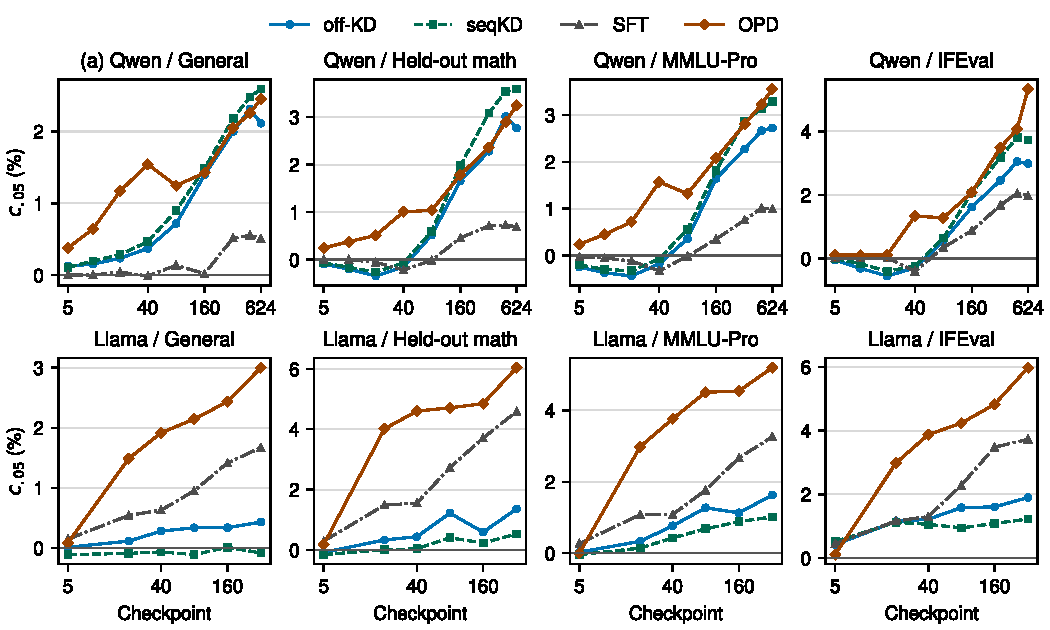
\includegraphics[width=\textwidth]{figures/supp_fig_full_domain_trajectories.pdf}
\caption{Complete equal-5 trajectories for the four frozen input domains in Qwen and
Llama. Panels retain the native checkpoint grids; no smoothing or interpolation is used.}
\label{fig:supp-full}
\end{figure*}

\subsection{Why Equal-5 Is Primary and Equal-7 Remains an Audit}

Query/key projections jointly form attention scores and are closer to routing, whereas
value/output and MLP projections more directly transform carried content. More
importantly, the empirical module audit finds heterogeneous q/k setting orderings and lower
baseline functional ranks. A change of only a few q/k directions can therefore receive
large relative weight. Excluding q/k is not a claim that they are irrelevant.

\begin{table}[t]
\centering
\small
\setlength{\tabcolsep}{4pt}
\begin{tabular}{lrr}
\toprule
Scope & q+k raw-rank share & relative share \\
\midrule
Qwen & 12.5\% & 46.4\% \\
Llama & 5.8\% & 25.8\% \\
Both models & 7.7\% & 32.2\% \\
\bottomrule
\end{tabular}
\caption{q/k share of early OPD contraction at $\varepsilon=.05$. The first column
counts removed directions; the second normalizes each module by its own baseline rank.
Neither is a causal or output-energy attribution.}
\label{tab:supp-qk}
\end{table}

Across $\varepsilon=.01,.025,.05,.10$, q+k account for
$17.1\%,11.9\%,7.7\%,3.2\%$ of raw rank-count contraction and
$35.8\%,33.8\%,32.2\%,27.4\%$ of baseline-relative contraction, respectively.
Thus q/k contribute few absolute directions, especially in Llama, but their relative
movement is not small. Equal-7 preserves the broad phenomenon while weakening
cross-model OPD dominance through this heterogeneity.

\begin{table*}[t]
\centering
\small
\setlength{\tabcolsep}{5pt}
\begin{tabular}{lrrlrrl}
\toprule
& \multicolumn{3}{c}{Qwen} & \multicolumn{3}{c}{Llama} \\
Module/aggregate & Strict & Tie & Offline & Strict & Tie & Offline \\
\midrule
q & 11 & 0 & 1 & 11 & 0 & 1 \\
k & 10 & 1 & 1 & 8 & 3 & 1 \\
v & 11 & 1 & 0 & 12 & 0 & 0 \\
o & 5 & 1 & 6 & 12 & 0 & 0 \\
gate & 12 & 0 & 0 & 12 & 0 & 0 \\
up & 12 & 0 & 0 & 12 & 0 & 0 \\
down & 11 & 0 & 1 & 12 & 0 & 0 \\
\midrule
equal-5 & 12 & 0 & 0 & 12 & 0 & 0 \\
equal-7 & 11 & 0 & 1 & 12 & 0 & 0 \\
\bottomrule
\end{tabular}
\caption{Complete module-level early ordering audit at $\varepsilon=.05$. Each model has
12 domain--checkpoint cells (four core domains at steps 20/40/80). ``Strict'' means OPD
has the largest contraction; ``Tie'' includes OPD at the maximum; ``Offline'' means an
offline setting is strictly larger. The heterogeneous Qwen o-projection shows that the
main equal-5 result is an aggregate mode-budget statement, not a claim of per-module
OPD dominance.}
\label{tab:supp-seven-modules}
\end{table*}

\subsection{Threshold, Continuous-Rank, Centering, and Layer Audits}

\begin{figure*}[t]
\centering
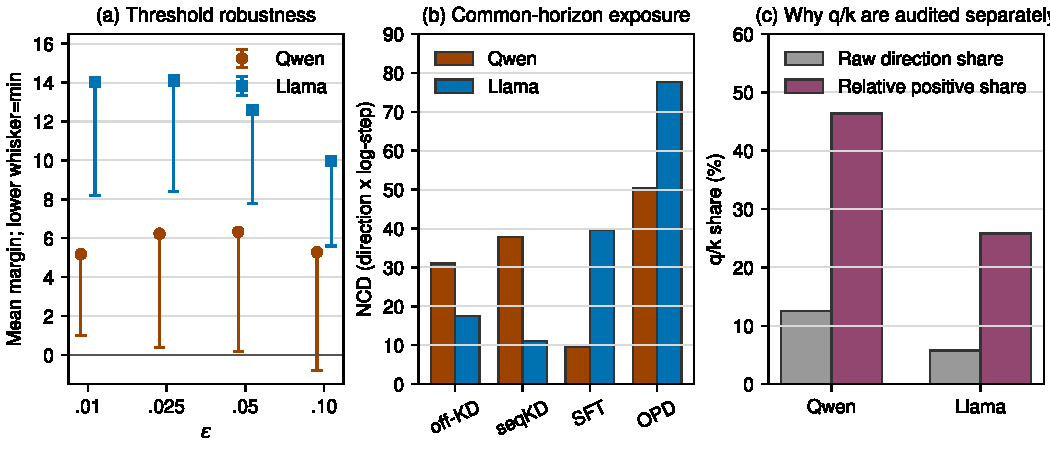
\includegraphics[width=\textwidth]{figures/supp_fig_robustness.pdf}
\caption{Robustness and decomposition audits. (a) Mean and minimum early OPD margin over
the four thresholds for both models. (b) Common-horizon normalized contraction depth
(NCD) by training setting and model. (c) Raw-rank and baseline-relative q/k shares.
Continuous-rank, centered-covariance, and layer audits are reported in the surrounding
text and Table~\ref{tab:supp-layers}.}
\label{fig:supp-robust}
\end{figure*}

The four audit classes named in the main paper have different formal coverage. Threshold
sensitivity covers both models: the shared early ordering holds in 48 of 48 Llama cells
and 47 of 48 Qwen cells across the four $\varepsilon$ values. Continuous state-spectrum
and centered-covariance audits are available for Llama, while layer audits cover both
models. They jointly preserve the reported conclusion under their stated coverage; this
does not assert uncomputed Qwen continuous-rank or centered-covariance results.

For Llama, OPD is deepest in every early model--domain--checkpoint cell under each of
$r_{.05}$, stable rank, and entropy effective rank. Mean early contractions for
OPD/SFT/off-KD/seqKD are $16.214/6.464/3.976/2.333$ directions for $r_{.05}$,
$.376/.165/.061/.029$ for stable rank, and
$11.991/5.145/2.097/1.160$ for entropy rank. Centering changes magnitudes to
$14.833/7.024/4.071/2.381$ directions but preserves the deepest setting in every
checkpoint--probe--threshold cell. Within centered results, the five primary modules
give 238 strict OPD orderings and two ties across 240 module-level cells; q and k are
substantially more heterogeneous.

The layer audit also rejects a midpoint-only artifact. Table~\ref{tab:supp-layers}
reports selected fully audited events, with positive values denoting contraction and
negative values denoting expansion. Qwen OPD differs from the offline paths at shallow,
middle, and deep locations, although the magnitude grows strongly with depth. For Llama
at step 160, the six-domain mean OPD contraction is deeper than off-KD at all three
layers, by $8.50$, $16.05$, and $31.45$ directions, respectively.

\begin{table*}[t]
\centering
\small
\setlength{\tabcolsep}{4pt}
\begin{tabular}{llrrrrrr}
\toprule
Model & Setting@step & \multicolumn{3}{c}{MMLU-Pro} &
\multicolumn{3}{c}{IFEval / six-domain mean} \\
& & Shallow & Middle & Deep & Shallow & Middle & Deep \\
\midrule
Qwen & OPD@40 & 1.857 & 10.000 & 40.429 & 2.571 & 5.857 & 54.571 \\
Qwen & SFT@40 & $-.714$ & $-2.714$ & 3.857 & $-.571$ & $-2.429$ & 1.429 \\
Qwen & off-KD@20 & .714 & $-3.143$ & 10.000 & $-.143$ & $-3.143$ & 14.429 \\
Qwen & seqKD@20 & .143 & $-2.714$ & 10.143 & $-.286$ & $-2.714$ & 14.143 \\
\midrule
Llama & OPD@160 & 19.12 & 20.88 & 40.81 & \multicolumn{3}{c}{six-domain mean} \\
Llama & off-KD@160 & 10.62 & 4.83 & 9.36 & \multicolumn{3}{c}{six-domain mean} \\
\bottomrule
\end{tabular}
\caption{Layer audit in contraction directions. Qwen shallow/middle/deep are L9/L18/L27;
the first numeric block is MMLU-Pro and the second is IFEval. Llama values are
six-domain means at L7/L14/L21 and are printed once in the first numeric block. The
Qwen offline controls use their available audited early event, so this table establishes
cross-layer presence rather than a same-step effect size.}
\label{tab:supp-layers}
\end{table*}

Native-space comparisons provide a separate construct check. At Llama OPD step 160,
normalized raw-activation effective rank changes by less than $.003$ across the audited
external domains and CKA remains between $.9997$ and $1.0000$, while functional rank at
the same module locations contracts by approximately 14--26 directions. Weight
principal-coordinate overlap, PABS, and NSS chiefly follow shared training progress or
small bare-spectrum movement in this LoRA setting and do not reproduce the same setting
ordering. These observations motivate the intermediate $WS$ coordinate; they do not
claim that activation- or weight-space diagnostics are generally uninformative.

\subsection{Exposure, Refresh, and Matched-Support Controls}

For Qwen $\alpha=.5$, eight of ten comparable early observations fall between off-KD and
OPD. For the flattened vector $z$ of equal-7 $\Delta r_{.05}$ values over the six frozen
sequence sets and steps 5/20/40/80/160, we compute
\begin{equation}
\widehat\lambda=
\frac{\langle z_{.5}-z_{\mathrm{off}},z_{\mathrm{OPD}}-z_{\mathrm{off}}\rangle}
{\|z_{\mathrm{OPD}}-z_{\mathrm{off}}\|_2^2}.
\end{equation}
This gives $\widehat\lambda=.376$ and Euclidean orthogonal residual
$\|z_{.5}-z_{\mathrm{off}}-\widehat\lambda
(z_{\mathrm{OPD}}-z_{\mathrm{off}})\|_2=.497$ directions. The comparison supports
ordered movement but not an exact one-dimensional dose law.

For Llama frozenSelf0-KD, OPD contracts more deeply on every fixed external probe at
every nonzero checkpoint. The five external paired margins remain positive throughout.
The paper reports only these fixed external measurement domains; the historical
self-generated response anchor is excluded from current means, figures, and claims.

Off-KD and seqKD isolate the target under identical sequences. Their equal-5 trajectories
have Pearson $.995$ and MAE $2.067$ directions in Qwen and Pearson $.944$ and MAE
$2.225$ in Llama. The close paths despite soft-versus-hard targets show that sequence
support can strongly organize this functional geometry; their different behavioral
endpoints show that it does not uniquely determine readout.

Per-domain Pearson/MAE (directions) are Qwen General $.995/1.13$, Math $.996/2.67$,
MMLU-Pro $.998/2.18$, and IFEval $.999/2.29$; Llama gives $-.771/2.53$,
$.971/1.73$, $.968/2.23$, and $.824/2.40$. Llama General has a different temporal
shape despite a small absolute budget difference, so pooled correlation cannot replace
the per-domain boundary.

\section{Output and Behavioral Readout}

\subsection{Whole-Completion Output Sensitivity}

Before introducing FAT regions, we computed cumulative KL and NLL on the entire fixed
reference completion. Within-setting correlations between contraction and cumulative KL are
$.954/.954/.901/.830$ for Llama OPD/SFT/off-KD/seqKD and
$.804/.717/.807/.820$ for Qwen. Absolute NLL correlations are
$.959/.928/.808/.751$ and $.710/.706/.729/.751$, respectively. After removing the
checkpoint-common setting mean, pooled KL correlations are $.703$ for Llama and $.176$ for
Qwen; absolute NLL correlations are $.744$ and $.286$. The unsigned relationship is
therefore visible without regional partitioning, while FAT localizes where it arises.

\subsection{Regional Unsigned Departure}

Within-setting Spearman correlations are high across most FAT regions. On MMLU-Pro,
Llama off-KD/OPD/seqKD/SFT correlations for answer are
$.943/1.000/1.000/1.000$; Qwen values are
$.933/.983/.933/.817$. On MATH, boxed-answer correlations are
$.943/1.000/.943/1.000$ for Llama and
$.867/.650/.883/.678$ for Qwen. Termination is similar except for Qwen SFT on MMLU
($.733$) and Qwen OPD on MATH ($.950$).

For Math CoT region $C$, off-KD/OPD/seqKD/SFT correlations are
$.943/.771/.943/1.000$ in Llama and $.867/.950/.883/.678$ in Qwen. All are
positive, extending the accumulated contraction--movement relation to reasoning tokens.

Checkpoint-demeaned correlations remain positive:
\begin{table}[t]
\centering
\small
\setlength{\tabcolsep}{3.5pt}
\begin{tabular}{llrrr}
\toprule
Model & Domain & \multicolumn{3}{c}{Region order} \\
\midrule
Llama & MMLU $F/A/T$ & .960 & .826 & .823 \\
Llama & MATH $C/B/T$ & .875 & .902 & .938 \\
Qwen & MMLU $F/A/T$ & .801 & .594 & .653 \\
Qwen & MATH $C/B/T$ & .573 & .440 & .595 \\
\bottomrule
\end{tabular}
\caption{Checkpoint-demeaned Spearman correlations. Each row follows the actual-region
order printed in column two. Demeaning removes only the contemporaneous four-setting
mean. The regional contrast $\mathrm{KL}_B-\mathrm{KL}_C$ is $-.209/-.183$ for
Llama/Qwen.}
\label{tab:supp-demean}
\end{table}

\subsection{Strict Construct Comparison}

The full checkpoint-held-out comparison contains 48 model--domain--target tasks. Llama
MMLU favors functional contraction over the best $p_k$ block in 11 of 13 $R^2$ tasks
and all 13 MAE tasks; Llama MATH gives 6 of 11 and 6 of 11. Qwen MMLU gives 7 of 13 and
6 of 13; Qwen MATH gives 5 of 11 and 5 of 11. Across all signed and unsigned targets,
mean held-out $R^2$ is $.435$ for functional contraction and $.421$ for $p_k$. The
advantage is therefore task-dependent, not universal.

On the 12 regional-KL targets emphasized in the paper, functional contraction has higher
$R^2$ on 10 and lower MAE on all 12. Adding $p_k$ to functional contraction improves
10 of 12 $R^2$ values by $.094$ on average and improves MAE on 9 of 12, directly
demonstrating complementarity.

On strict 64-cell common grids for both models, held-out metrics for raw activation
$A$, functional contraction $C_5$, weight placement $P_{k,5}$, and combinations are:
\begin{table*}[t]
\centering
\small
\setlength{\tabcolsep}{3.5pt}
\begin{tabular}{llrrrrr}
\toprule
Model & Target & $A$ & $C_5$ & $P_{k,5}$ & $A+C_5$ & $P_{k,5}+C_5$ \\
\midrule
Llama & Cumulative KL $R^2$ & .104 & \textbf{.720} & -.349 & .722 & .433 \\
 & Absolute NLL $R^2$ & .181 & \textbf{.738} & .436 & .651 & .728 \\
 & Signed NLL $R^2$ & .022 & \textbf{.541} & -.364 & .373 & -.008 \\
 & OPD AUC & .556 & .743 & .688 & \textbf{.751} & .724 \\
Qwen & Cumulative KL $R^2$ & -.575 & \textbf{.344} & .052 & .075 & -.003 \\
 & Absolute NLL $R^2$ & .112 & .247 & .261 & .033 & \textbf{.299} \\
 & Signed NLL $R^2$ & -.284 & .278 & -.264 & \textbf{.328} & .183 \\
 & OPD AUC & .595 & .708 & .521 & \textbf{.712} & .667 \\
\bottomrule
\end{tabular}
\caption{Nested checkpoint-held-out comparison on strict 64-cell grids for both models.
Standardization and regularization selection use outer-training checkpoints only.
Qwen absolute NLL is the strict-$p_k$ counterexample. Qwen $C_5$ has higher OPD AUC
but log-loss 1.305, so the ranking result is not a calibration advantage.}
\label{tab:supp-rr5}
\end{table*}

\begin{table*}[t]
\centering
\small
\begin{minipage}[t]{0.615\textwidth}
\centering
\textit{A. Length and termination}\\[2pt]
\setlength{\tabcolsep}{2.5pt}
\begin{tabular}{@{}rrrr@{}}
\toprule
Step & Response tokens & EOS & Truncated \\
\midrule
20 & $238.9\ [139.4,333.1]$ & $-.184\ [-.246,-.124]$ & $.184\ [.124,.246]$ \\
40 & $-3136.0\ [-3648.0,-2603.1]$ & $.180\ [.118,.242]$ & $-.180\ [-.242,-.118]$ \\
80 & $536.5\ [26.5,1073.9]$ & $-.166\ [-.230,-.106]$ & $.166\ [.106,.230]$ \\
160 & $1126.1\ [627.4,1630.3]$ & $-.190\ [-.250,-.132]$ & $.190\ [.132,.250]$ \\
\bottomrule
\end{tabular}
\end{minipage}\hfill
\begin{minipage}[t]{0.38\textwidth}
\centering
\textit{B. Repetition and answer format}\\[2pt]
\setlength{\tabcolsep}{2.5pt}
\begin{tabular}{@{}rrr@{}}
\toprule
Step & 4-gram repetition & Boxed \\
\midrule
20 & $-.043\ [-.076,-.011]$ & $-.064\ [-.122,-.006]$ \\
40 & $-.324\ [-.364,-.283]$ & $.374\ [.318,.430]$ \\
80 & $-.070\ [-.112,-.029]$ & $.192\ [.132,.248]$ \\
160 & $.011\ [-.030,.050]$ & $-.062\ [-.118,-.008]$ \\
\bottomrule
\end{tabular}
\end{minipage}
\caption{Mean paired OPD-minus-frozenSelf0-KD differences with 95\% paired bootstrap
intervals on the same 500 MATH500 items. Positive values mean larger/more frequent under
OPD. Distinct-2, omitted for width, likewise changes sign across checkpoints. These are
readout descriptors, not independently randomized mediators.}
\label{tab:supp-refresh-ci}
\end{table*}

\subsection{Signed Readout and Behavioral Boundary}

After checkpoint demeaning, correlations between contraction and signed regional NLL
contrasts are model-dependent. Llama MMLU gives
$.822/.500/.368/.788$ for $\Delta A,\Delta F,F-A,\Delta T$, and Llama MATH gives
$.144/-.296/.888/.927$ for $\Delta B,B-C,\Delta C,\Delta T$. Qwen gives
$.417/.394/.145/.481$ and $.403/.291/.529/-.079$, respectively. These mixed signs
explain why unsigned output movement is the more stable functional-spectrum relation.

The same boundary appears in free generation. The MMLU format contrast $F-A$ correlates
with the flexible--strict accuracy gap by
$-.543,-.029,.829,-.086$ for Llama OPD/off-KD/seqKD/SFT and
$-.217,.717,.717,.667$ for Qwen. No single signed regional variable mediates behavior
across settings and models in these observational comparisons; the analysis does not
identify a causal mediator.

\subsection{Mechanistic and Generalization Audits}

Several secondary audits constrain interpretation:
\begin{itemize}
    \item Qwen Math-CoT training and held-out probes have Pearson $.994$, Spearman $.977$,
    and MAE $.813$ directions across matched setting--checkpoint cells. This is
    inconsistent with a purely training-item-specific account of the geometry.
    \item On the fixed 128-item NuminaMath-1.5 geometry probe, seven-module contraction
    at steps 40/160/624 is $27.57/48.14/75.00$ directions for OPD. OPD is deepest at
    step 40, while off-KD reaches $53.71$ at step 160 and off-KD/seqKD reach
    $93.57/93.14$ at step 624. The probe and a separate 200-item zero-shot evaluation
    split are prompt-deduplicated against Math-CoT training fingerprints, mutually
    disjoint, and frozen with seed 20260725. This audit limits endpoint generalization
    while preserving the shared early claim.
    \item Zeroing Qwen off-KD adapters at layers 12--17 reduces strict-format failure by
    $.200$, with essentially unchanged flexible accuracy and a $-.005$ math-accuracy
    change. This supports a readout-channel interpretation without proving one mechanism.
    \item Qwen OPD moves answer-position probability mass outside legal option tokens:
    legal mass falls from $.1915$ to $.1301$, while entropy rises from $2.402$ to $4.746$.
    The failure is not merely indecision among legal choices.
    \item A 500-item paired comparison for Llama OPD minus frozenSelf0-KD gives
    checkpoint-varying signs for response length, EOS, truncation, repetition,
    distinct-2, and boxed-answer presence. Table~\ref{tab:supp-refresh-ci} reports the
    principal 2,000-resample paired intervals. This sign instability does not identify a
    mediator; refresh remains a bundle-level intervention.
\end{itemize}

\subsection{Artifact and Reporting Boundary}

All plots use the frozen CSV artifacts rather than values transcribed from prose. Figures
are vector PDF at final layout size; visible text is at least 9\,pt, line widths are
at least 0.5\,pt, and fonts are embedded without Type 3. The manuscript does not use
plot-side color as the sole carrier of meaning: setting identity is repeated through
markers, line styles, labels, or table entries.

The supplement reports estimator and cell-level robustness, but it does not manufacture
seed uncertainty. The separately uploaded anonymous reproducibility artifact is a
source-code package containing experiment and analysis entry points, dependency files,
registry schemas and templates, and file-level checksums for the included source. Model
checkpoints, rollout and activation caches, generated result tables, run-specific
manifests, and frozen sample-ID inventories are not bundled.

\end{document}
